\documentclass[11pt,a4paper]{article}
\usepackage[margin=2.4cm]{geometry}
\usepackage[T1]{fontenc}
\usepackage[utf8]{inputenc}
\usepackage{lmodern}
\DeclareUnicodeCharacter{03BB}{\ensuremath{\lambda}}
\DeclareUnicodeCharacter{00E9}{\'e}
\DeclareUnicodeCharacter{00E3}{\~a}
\DeclareUnicodeCharacter{00F3}{\'o}
\usepackage{amsmath,amssymb}
\usepackage{booktabs,graphicx,caption,float,array,tabularx}
\usepackage{xcolor}
\usepackage[numbers]{natbib}
\usepackage[colorlinks=true,linkcolor=blue!50!black,citecolor=blue!50!black,urlcolor=blue!50!black]{hyperref}
\usepackage{cleveref}
\captionsetup{font=small,labelfont=bf}
\setlength{\parskip}{4pt}
\graphicspath{{figs/}}
\newcommand{\R}{\mathrm{RWR}}
\newcommand{\pa}{@10}

\title{\textbf{A Hybrid Recommender on a User--Film--Content Graph}\\[2pt]
\large AIM608 Networks and Semantics I --- End-term Project 4}
\author{Shikhar Mutta (MT2025114), Hasini Yamsani (BT2024133), D.\ Sreeteja (BT2024160)\\ Mentor: \emph{[mentor]}}
\date{\today}

\begin{document}
\maketitle

\begin{abstract}
\noindent We build a film recommender on MovieLens \emph{latest-small} in which users, films and content are one graph: ratings link users to films and sentence-embedding similarity links films to films. A random walk with restart (personalised PageRank) on this graph reaches films that similar users liked and films that are similar to those. We implement item-based collaborative filtering, random walk with restart (RWR), a content-only model, a graph hybrid whose content-edge weight $\lambda$ can be varied, a popularity-discounted walk, a score-level late-fusion baseline and a node2vec-style embedding method, and compare them under a protocol with a train/validation/test split made \emph{before} any edge is built. On warm films, a small content weight ($\lambda=0.1$) raises precision@10 from $0.174$ to $0.184$ (gain in each of 3 splits) and accuracy collapses when content dominates ($\lambda\ge0.3$). On \emph{cold-start} films with no ratings, the collaborative methods are at chance, while the hybrid has $3.4\times$ the recall of chance (recall@10 $0.088$ vs.\ $0.026$) already at $\lambda=0.02$. All methods recommend mostly popular films; a popularity discount gives the best warm accuracy (precision@10 $0.197$). Taste communities found by projecting onto users differ strongly in genre mix (permutation $p<10^{-3}$).
\end{abstract}

\tableofcontents


%--------------------------------------------------------------------------------------
\section{Introduction and problem}
A recommender suggests films that a user may like. \emph{Collaborative filtering} (CF) uses ratings: it recommends what users with similar taste liked, but it cannot recommend a film that nobody has rated. \emph{Content-based filtering} uses what a film is about (genres, tags), so it can recommend a new film, but it ignores what users liked. Both fit in a single network (\cref{fig:schema}): \emph{ratings} join users to films, and \emph{content similarity} joins films to films. A random walk on this graph reaches films that similar users liked, and films similar to those.

\begin{figure}[H]\centering
\begin{tabular}{@{}c@{\hspace{.4cm}}c@{}}
\begin{minipage}{.5\linewidth}\small
\textbf{Nodes:} users ($610$) and films ($9{,}742$).\\
\textbf{Rating edge:} user $\leftrightarrow$ film, weight = rating ($\text{80\,\%}$ of $100{,}836$ in training).\\
\textbf{Content edge:} film $\leftrightarrow$ film if one is among the $k=20$ most similar films of the other (cosine of sentence embeddings).\\
\textbf{Walk:} from a film follow a content edge with probability $\lambda$, a rating edge with $1-\lambda$; restart at the user with probability $c$.
\end{minipage}
&
\begin{minipage}{.4\linewidth}\centering
$\displaystyle r\;\leftarrow\;(1-c)\,P_\lambda\,r+c\,e_u$\\[6pt]
{\small $P_\lambda=\begin{bmatrix}0&P_{UF}(1-\lambda)\\ P_{FU}&\lambda\,P_{FF}\end{bmatrix}$}
\end{minipage}
\end{tabular}
\caption{The network and the walk. $P_{FU}$: user$\to$film transitions (rating-weighted); $P_{UF}$: film$\to$user; $P_{FF}$: film$\to$film (content, cosine-weighted); a film with no ratings uses $\lambda=1$.}\label{fig:schema}
\end{figure}

\paragraph{Questions.} (Q1) How accurate are item-based CF, RWR and the hybrid (precision/recall@10, hidden 20\,\% of each user's ratings)? (Q2) How well do the methods recommend films with \emph{no} ratings (cold start)? (Q3) Do the methods recommend mostly popular films? (Q4) Do communities of users follow genres? (Q5) At what content weight does accuracy peak? In addition: (Q6) does a graph hybrid beat a simple score-level blend, and (Q7) can a new unrated film be matched to users in the demo?

\paragraph{Contributions.} Besides the requested models, (i)~we verify the RWR implementation three independent ways (power iteration, exact linear solve, Monte-Carlo walk); (ii)~we show that popularity bias of the walk can be removed with a degree discount and that this is the single largest accuracy gain on warm films; (iii)~we compare the graph hybrid to a late-fusion baseline and to node2vec; (iv)~we measure cold start in two directions (rank cold films per user; rank users per cold film); (v)~all hyper-parameters are chosen on a validation split, and all results are averaged over three random splits.

%--------------------------------------------------------------------------------------
\section{Data}
We use MovieLens \emph{latest-small} \citep{harper2015}: $100{,}836$ ratings (0.5--5 stars) of $9{,}724$ rated films ($9{,}742$ in the catalogue) by $610$ users, with genres and $3{,}683$ user tag applications. Density is only $1.7\,\%$ and the data are very skewed (\cref{fig:data}): the top $10\%$ most-rated films receive $60\%$ of all ratings, the median film has $3$ ratings and $62\%$ of films have fewer than $5$. This is why popularity and cold start matter. A film is \emph{liked} if rated $\ge4$.

\begin{figure}[H]\centering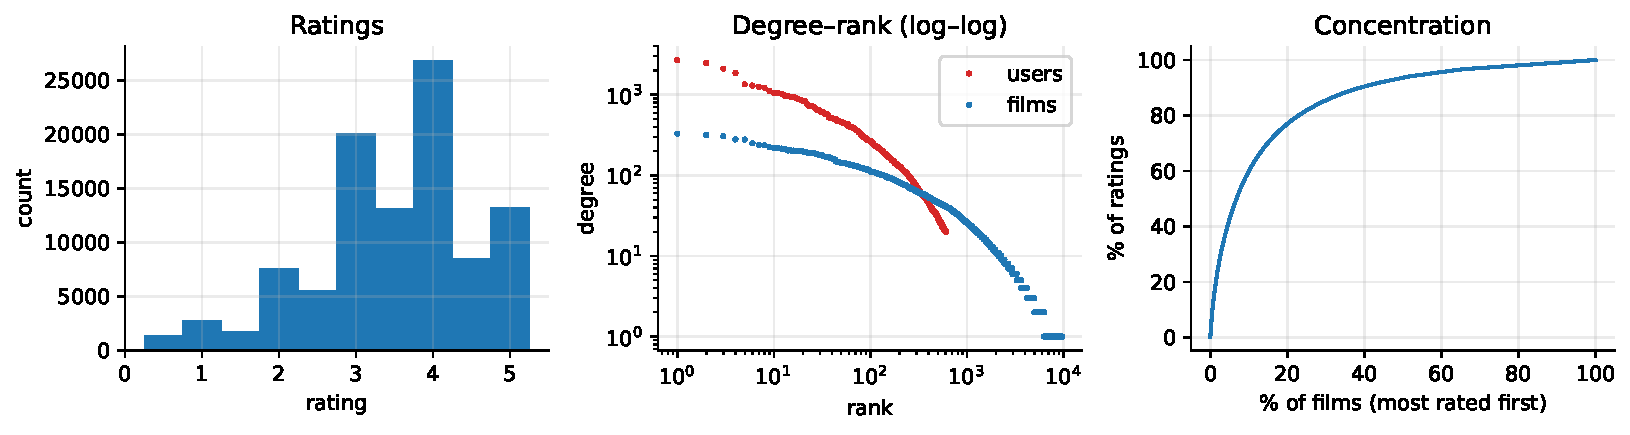
\includegraphics[width=\linewidth]{fig_data}
\caption{Rating distribution, degree--rank plot (log--log) and concentration of ratings.}\label{fig:data}\end{figure}

%--------------------------------------------------------------------------------------
\section{Methods}\label{sec:methods}
Let $A\in\mathbb R^{n_U\times n_I}$ be the training rating matrix (rating as weight). All models output a score for every user--film pair; films the user rated in training are excluded from recommendations.

\paragraph{Item-based CF \citep{linden2003}.} Project the user--film graph onto films: $S=\tilde A^{\top}\tilde A$ where the columns of $A$ are $L_2$-normalised ($S$ is the cosine similarity of rating columns; raw co-rating counts would favour popular films). The score of film $i$ for user $u$ is $\sum_{j\in L_u}S_{ji}$ where $L_u$ is the set of films $u$ liked.

\paragraph{Random walk with restart \citep{fouss2007,page1999}.} Build the symmetric bipartite graph on users$\,\cup\,$films, with transition matrix $P$ (column-stochastic, edge weight = rating). For a user $u$ the personalised PageRank vector is the solution of $r=(1-c)Pr+c\,e_u$, computed by power iteration for all users at once. Films are ranked by their entry in $r$. This is the ``ratings only'' model ($\lambda=0$).

\paragraph{Content similarity.} Each film is a text ``\emph{title. Genres: \dots\ Tags: \dots}''. It is embedded with \texttt{sentence-transformers} (\texttt{all-MiniLM-L6-v2}, 384 dim; \citealt{reimers2019}), vectors are normalised, and each film is linked to its $k=20$ most cosine-similar films (graph symmetrised, weight = cosine). \Cref{tab:nn} shows that the neighbours make sense (\emph{Toy Story}$\to$\emph{Toy Story 3, 2, A Bug's Life}); the genre Jaccard overlap of a film and its nearest neighbour is $0.63$ vs.\ $0.17$ for random pairs. Tags exist for only about $1.6$k films, so many films have thin descriptions (e.g. \emph{3 Idiots} has no tags and is matched with \emph{The Idiots} by its title: a limitation of a text-only content model).

\begin{table}[H]\centering\small
\begin{tabular}{ll}\toprule
Film & Nearest content neighbours (cosine)\\\midrule
Toy Story (1995) & Toy Story 3 (.88), Toy Story 2 (.85), Toys (.82), A Bug's Life (.82), Shrek (.77)\\
3 Idiots (2009) & The Idiots (.88), Smart People (.81), Idiots and Angels (.80), Guess Who (.79)\\
Like Stars on Earth (2007) & O (.80), Ju Dou (.79), W. (.78), L.I.E. (.77), Solas (.77)\\\bottomrule
\end{tabular}\caption{Examples of content neighbours.}\label{tab:nn}\end{table}

\paragraph{Content only.} A non-graph baseline: cosine between the film embedding and the user's profile (rating-weighted mean embedding of liked films).

\paragraph{The hybrid.} Run the walk on the graph with both edge types. A film node follows a content edge with probability $\lambda$ and a rating edge with probability $1-\lambda$; a user follows a rating edge. Thus $\lambda$ is the weight of content edges against rating edges. A film with no ratings has no rating edge, so it always uses content edges ($\lambda_i=1$), which is how a cold film becomes reachable (it receives probability mass from its content neighbours and passes it back to them).

\paragraph{Other approaches.} (a)~\emph{Popularity discount:} the stationary mass of the walk grows with film degree, so scores are divided by $(1+n_i)^{\beta}$ ($n_i$ = number of training ratings). (b)~\emph{Late fusion:} $(1-\alpha)\,\text{minmax}(\text{item-CF})+\alpha\,\text{minmax}(\text{content})$, a non-graph hybrid used as a baseline. (c)~\emph{node2vec} \citep{grover2016}: random walks on the hybrid graph, skip-gram with negative sampling (own PyTorch implementation, 64 dim, 5 walks of length 30 per node, window 4; walks are first-order, i.e.\ $p=q=1$, which is DeepWalk \citep{perozzi2014}); score = cosine of user and film embeddings.

%--------------------------------------------------------------------------------------
\section{Experimental protocol}
\begin{itemize}\setlength\itemsep{0pt}
\item \textbf{Split before edges are built.} For every user $20\%$ of the ratings (at least one) are hidden as the test set; all graphs, similarity matrices, popularity counts and user profiles are built from the remaining $80\%$ only (no test leakage). \emph{Relevant} films = hidden films rated $\ge4$; precision@10, recall@10 and NDCG@10 are averaged over users with at least one relevant film ($\approx600$).
\item \textbf{Validation.} Hyper-parameters --- restart probability $c\in\{0.3,0.5,0.7\}$, content weight $\lambda$, discount $\beta$, fusion weight $\alpha$ --- are chosen on a validation split taken from the training set (15\,\% of each user's training ratings). The test set is never used for tuning. The $\lambda$ sweep on test (Q5) is reported separately, as an analysis. $k=20$ content neighbours unless stated.
\item \textbf{Repetitions.} All numbers are mean $\pm$ standard deviation over \textbf{3 random splits} (seeds 0, 1, 2).
\item \textbf{Cold start.} $10\%$ of the films that have $\ge5$ ratings ($365$ films) have \emph{all} their ratings removed from training. For each user we rank only these cold films (the ``new releases'' shelf), and relevant = liked in the hidden data. A \emph{Random} ranking is the reference. Reverse direction: for each cold film we rank users (by the film's rank within each user's cold list) and report precision@10 over users who liked it and its lift over the film's base rate.
\item \textbf{Popularity.} Share of recommended films outside the top $10\%$ most-rated films (training counts), plus catalogue coverage.
\end{itemize}
Code: \texttt{src/hybrid\_rec.py}, notebook \texttt{hybrid\_recommender.ipynb} (contains the code behind every number and figure).

%--------------------------------------------------------------------------------------
\section{Results}

\subsection{Warm-up: personalised PageRank on the user--film graph}
For user 105, who liked \emph{3 Idiots} and \emph{Taare Zameen Par}, we computed personalised PageRank by power iteration on the user--film graph alone ($c=0.15$). The iteration converges geometrically at rate $1-c$ (175 iterations to an $L_1$ change below $10^{-12}$). It agrees with the exact solution $r=c(I-(1-c)P)^{-1}e_u$ up to $5\cdot10^{-15}$ and matches the visit frequencies of a simulated random walk (Spearman $0.95$ over films; \cref{fig:warm}). As required, films rated highly by similar users rank near the top: the $30$ users the walker visits most rated the walk's top-10 films $3.81$ on average vs.\ $3.11$ for ten random unseen films, and all ten were rated by them.

\begin{figure}[H]\centering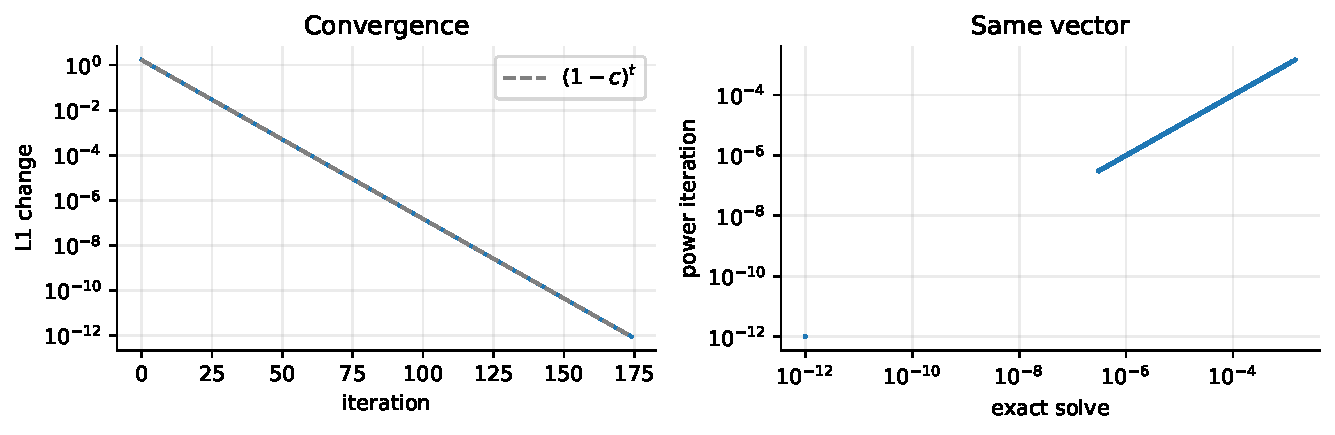
\includegraphics[width=.8\linewidth]{fig_warmup}
\caption{Warm-up. Left: convergence of the power iteration against $(1-c)^t$. Right: power iteration vs.\ exact solve.}\label{fig:warm}\end{figure}

\subsection{Accuracy (Q1)}
\begin{table}[H]\centering\small
\begin{tabular}{lccc}
\toprule
 & precision@10 & recall@10 & NDCG@10 \\
\midrule
Popularity & 0.119 ± 0.003 & 0.097 ± 0.001 & 0.157 ± 0.003 \\
Item-based CF & 0.174 ± 0.004 & 0.169 ± 0.003 & 0.231 ± 0.002 \\
Content only (profile) & 0.003 ± 0.001 & 0.006 ± 0.002 & 0.007 ± 0.002 \\
RWR (ratings only) & 0.174 ± 0.004 & 0.169 ± 0.004 & 0.235 ± 0.005 \\
RWR + popularity discount & 0.197 ± 0.005 & 0.189 ± 0.001 & 0.266 ± 0.006 \\
Late fusion (CF+content) & 0.172 ± 0.002 & 0.169 ± 0.003 & 0.232 ± 0.001 \\
Hybrid RWR & 0.184 ± 0.005 & 0.179 ± 0.003 & 0.251 ± 0.006 \\
Hybrid RWR + popularity discount & 0.187 ± 0.005 & 0.184 ± 0.004 & 0.256 ± 0.007 \\
node2vec on hybrid graph & 0.045 ± 0.003 & 0.068 ± 0.005 & 0.067 ± 0.006 \\
\bottomrule
\end{tabular}

\caption{Hide 20\,\% of each user's ratings: mean $\pm$ s.d.\ over 3 splits, $k=10$. Hyper-parameters chosen on validation ($c=0.7$; hybrid $\lambda=0.1$ in all splits; discount $\beta=0.5$).}\label{tab:acc}\end{table}

\begin{figure}[H]\centering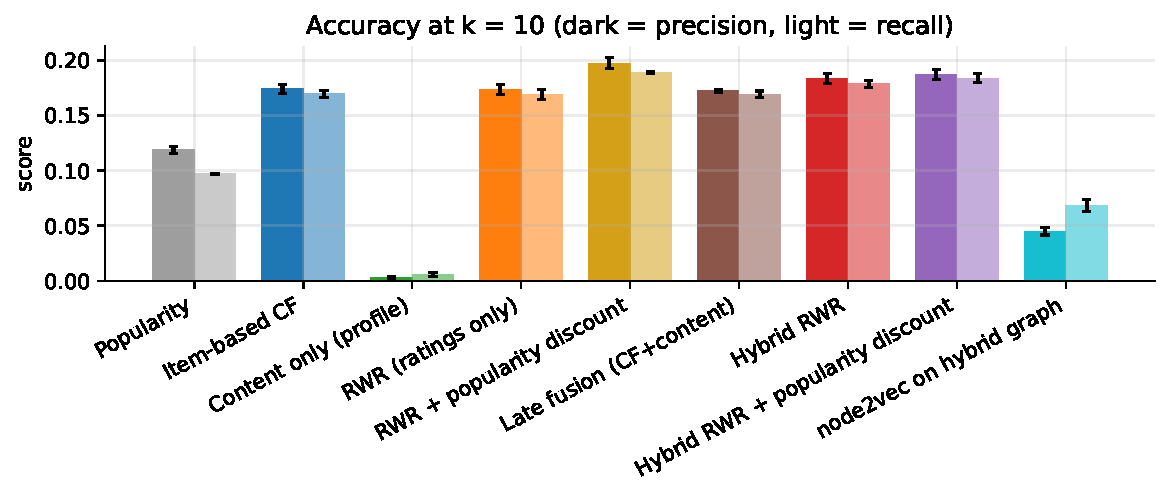
\includegraphics[width=.8\linewidth]{fig_accuracy}
\caption{precision@10 (dark) and recall@10 (light).}\label{fig:acc}\end{figure}

Item-based CF and the ratings-only RWR are equally accurate (precision@10 $0.174$) and clearly beat the popularity baseline ($0.119$). The hybrid at $\lambda=0.1$ improves on the ratings-only walk by $+0.010$ ($+5.8\%$ relative; the gain is positive in each split: $+0.008,+0.009,+0.014$, with a split-to-split s.d.\ of $0.005$ on the level) and the largest single gain comes from discounting popularity ($0.197$). A \emph{content-only} model is almost useless for warm accuracy ($0.003$): it recommends obscure films with similar text, which almost no user rated in the hidden set. The score-level \emph{late fusion} baseline does not improve on item-CF ($0.172$, with $\alpha$ tuned to a very small value), whereas the \emph{graph} hybrid does, so \textbf{(Q6)} mixing at the graph level, where content edges let the walk pass through films and users, is more useful than blending final scores. The node2vec model is much weaker ($0.045$); it recommends obscure films (tail share $0.70$) because skip-gram embeddings capture neighbourhoods rather than the stationary weights that RWR uses. With the budget used here (2 epochs, 64 dimensions) it is not competitive on warm films, but it is competitive on cold films (below).

Jointly discounting popularity \emph{and} using content in the hybrid ($0.187$) was chosen on validation with a small $\beta$ ($0.0$--$0.2$) because larger $\beta$ over-promotes the obscure films that content edges bring in. Hence on warm films the two remedies against popularity bias (a discount and content edges) do not add up in our experiments; we discuss this in \cref{sec:disc}.

\subsection{The weight of content (Q5)}
\begin{figure}[H]\centering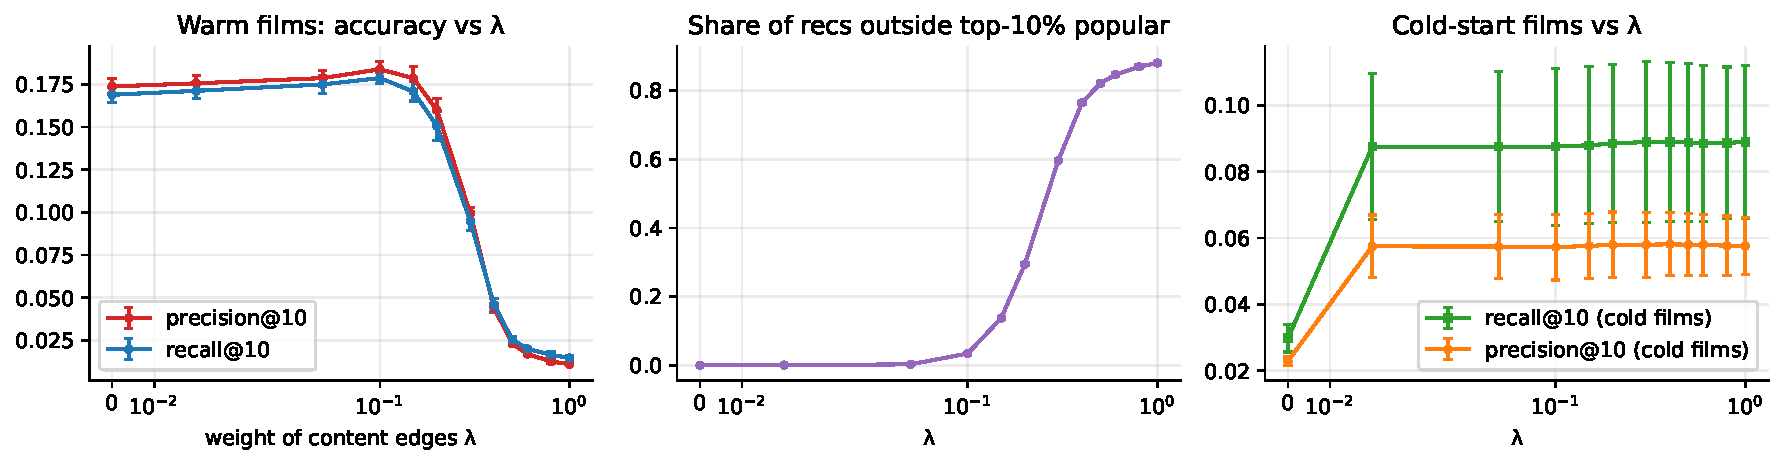
\includegraphics[width=\linewidth]{fig_lambda}
\caption{Effect of the weight of content edges $\lambda$ (symlog axis). Left: warm accuracy. Middle: share of recommendations outside the top-10\,\% popular films. Right: cold-start films.}\label{fig:lam}\end{figure}
\begin{table}[H]\centering\small\begin{tabular}{lcccc}
\toprule
λ & precision@10 & recall@10 & tail share & cold recall@10 \\
\midrule
0 & 0.1737 ± 0.0044 & 0.1688 & 0.000 & 0.0298 \\
0.02 & 0.1755 ± 0.0047 & 0.1711 & 0.000 & 0.0875 \\
0.05 & 0.1786 ± 0.0046 & 0.1749 & 0.003 & 0.0876 \\
0.1 & 0.1838 ± 0.0046 & 0.1786 & 0.034 & 0.0876 \\
0.15 & 0.1785 ± 0.0069 & 0.1708 & 0.137 & 0.0880 \\
0.2 & 0.1599 ± 0.0068 & 0.1505 & 0.295 & 0.0885 \\
0.3 & 0.0993 ± 0.0037 & 0.0948 & 0.596 & 0.0890 \\
0.4 & 0.0440 ± 0.0025 & 0.0458 & 0.764 & 0.0889 \\
0.5 & 0.0231 ± 0.0014 & 0.0254 & 0.821 & 0.0888 \\
0.6 & 0.0170 ± 0.0005 & 0.0200 & 0.846 & 0.0886 \\
0.8 & 0.0126 ± 0.0009 & 0.0166 & 0.870 & 0.0887 \\
1 & 0.0110 ± 0.0006 & 0.0147 & 0.880 & 0.0890 \\
\bottomrule
\end{tabular}
\caption{Sweep of $\lambda$ (hybrid, $c=0.7$, $k=20$; mean over 3 splits; $\pm$ is the s.d.\ of precision).}\label{tab:lam}\end{table}

\textbf{Accuracy on warm films peaks at $\lambda\approx0.1$ in all 3 splits} (precision@10 $0.184$ vs.\ $0.174$ at $\lambda=0$), is flat for $0.05\le\lambda\le0.15$, and then \emph{falls sharply}: at $\lambda=0.3$ it is $0.099$ and for $\lambda\ge0.5$ below $0.025$, where recommendations are almost purely content-driven (tail share $>0.8$). Content edges therefore act as a gentle regulariser: a little content smooths the sparse rating graph, but too much lets the walker leak into obscure content-similar films that nobody rated. In contrast, \textbf{for cold films a very small content weight already suffices}: cold recall@10 jumps from $0.030$ ($\lambda=0$, chance) to $0.0875$ at $\lambda=0.02$ and then stays flat ($\approx0.088$--$0.089$). So the same hybrid with $\lambda\approx0.1$ is simultaneously near-best for warm and for cold films.

Robustness (hybrid, $\lambda=0.1$): the restart probability matters ($c=0.15$: $0.154$; $0.5$: $0.176$; $0.7$: $0.184$; $0.85$: $0.168$) and the number of content neighbours much less ($k=5$: $0.177$, $10$: $0.186$, $20$: $0.184$, $40$: $0.181$); see \cref{tab:ck}. A large restart probability keeps the walk close to the user, which suits sparse data.

\begin{table}[H]\centering\small
\begin{minipage}{.4\linewidth}\centering\begin{tabular}{lcc}
\toprule
k & precision@10 & recall@10 \\
\midrule
5 & 0.1768 & 0.1596 \\
10 & 0.1861 & 0.1765 \\
20 & 0.1838 & 0.1786 \\
40 & 0.1805 & 0.1765 \\
\bottomrule
\end{tabular}
\end{minipage}\hfill
\begin{minipage}{.4\linewidth}\centering\begin{tabular}{lcc}
\toprule
c & precision@10 & recall@10 \\
\midrule
0.15 & 0.1539 & 0.1425 \\
0.3 & 0.1662 & 0.1583 \\
0.5 & 0.1764 & 0.1725 \\
0.7 & 0.1838 & 0.1786 \\
0.85 & 0.1677 & 0.1579 \\
\bottomrule
\end{tabular}
\end{minipage}
\caption{Number of content neighbours $k$ (left) and restart probability $c$ (right).}\label{tab:ck}\end{table}

\subsection{Cold start (Q2)}
\begin{table}[H]\centering\scriptsize\resizebox{\linewidth}{!}{\begin{tabular}{lccccc}
\toprule
 & precision@10 & recall@10 & NDCG@10 & user-side P@10 & user-side lift \\
\midrule
Random & 0.021 ± 0.001 & 0.026 ± 0.004 & 0.025 ± 0.002 & 0.019 ± 0.003 & 1.03 ± 0.30 \\
Item-based CF & 0.023 ± 0.001 & 0.029 ± 0.003 & 0.029 ± 0.003 & 0.023 ± 0.004 & 1.28 ± 0.29 \\
RWR (ratings only) & 0.023 ± 0.001 & 0.030 ± 0.004 & 0.030 ± 0.002 & 0.023 ± 0.004 & 1.28 ± 0.29 \\
Content only (profile) & 0.025 ± 0.002 & 0.035 ± 0.006 & 0.037 ± 0.001 & 0.032 ± 0.005 & 2.28 ± 0.26 \\
Hybrid RWR & 0.057 ± 0.010 & 0.088 ± 0.024 & 0.082 ± 0.019 & 0.044 ± 0.004 & 2.94 ± 0.39 \\
node2vec on hybrid graph & 0.053 ± 0.001 & 0.079 ± 0.002 & 0.079 ± 0.002 & 0.054 ± 0.004 & 3.20 ± 0.29 \\
\bottomrule
\end{tabular}
}
\caption{Cold start: 10\,\% of the films ($365$) have all ratings hidden. Left block: rank the $365$ cold films for each user. Right block: rank users for each cold film (lift over the base rate; random $\approx1$).}\label{tab:cold}\end{table}
\begin{figure}[H]\centering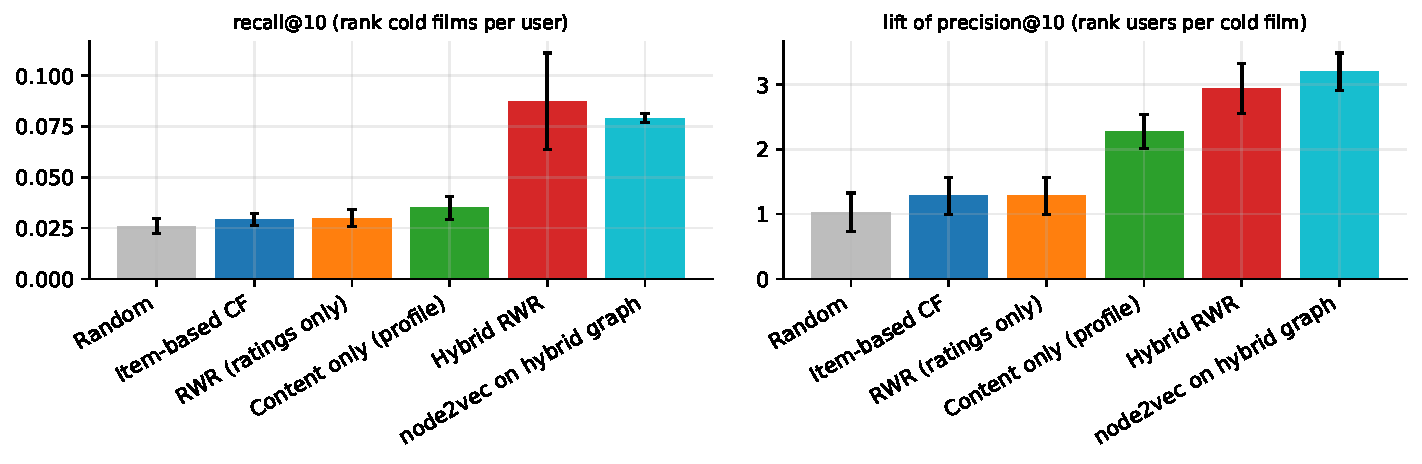
\includegraphics[width=.85\linewidth]{fig_cold}
\caption{Cold-start performance.}\label{fig:cold}\end{figure}

As expected, the collaborative methods (item-CF and ratings-only RWR) are at chance on cold films (precision@10 $0.023$ vs.\ $0.021$ for Random). The content-profile model is only slightly better ($0.025$) because users' liked films are dominated by popular genres. The \textbf{hybrid has recall@10 $0.088$, $3.4\times$ the recall of chance ($0.026$)}, and precision@10 $0.057$ vs.\ $0.021$. In the reverse direction (which users should get a new film), the hybrid has a lift of $2.9$ over random; node2vec on the hybrid graph, which is poor on warm films, is the best here ($3.2$), consistent with it encoding content neighbourhoods. The cold-start variance is larger because only $\approx365$ films have a few likers each.

\subsection{Popularity (Q3)}
\begin{table}[H]\centering\scriptsize\resizebox{\linewidth}{!}{\begin{tabular}{lcccc}
\toprule
 & precision@10 & outside top-10\% popular & catalogue coverage & mean log(1+\#ratings) \\
\midrule
Popularity & 0.119 & 0.000 ± 0.000 & 0.005 ± 0.000 & 5.265 ± 0.001 \\
Item-based CF & 0.174 & 0.029 ± 0.003 & 0.050 ± 0.003 & 4.603 ± 0.008 \\
Content only (profile) & 0.003 & 0.949 ± 0.008 & 0.034 ± 0.001 & 1.353 ± 0.049 \\
RWR (ratings only) & 0.174 & 0.000 ± 0.000 & 0.012 ± 0.001 & 5.167 ± 0.001 \\
RWR + popularity discount & 0.197 & 0.052 ± 0.004 & 0.049 ± 0.000 & 4.797 ± 0.011 \\
Late fusion (CF+content) & 0.172 & 0.033 ± 0.002 & 0.052 ± 0.001 & 4.580 ± 0.016 \\
Hybrid RWR & 0.184 & 0.034 ± 0.002 & 0.028 ± 0.001 & 5.002 ± 0.007 \\
Hybrid RWR + popularity discount & 0.187 & 0.046 ± 0.010 & 0.032 ± 0.004 & 4.927 ± 0.059 \\
node2vec on hybrid graph & 0.045 & 0.704 ± 0.006 & 0.287 ± 0.002 & 2.020 ± 0.025 \\
\bottomrule
\end{tabular}
}
\caption{Popularity and diversity of the recommendations ($k=10$): fraction of recommended films outside the top $10\%$ most-rated films, catalogue coverage and mean $\log(1+\#\text{ratings})$ of recommended films.}\label{tab:pop}\end{table}
\begin{figure}[H]\centering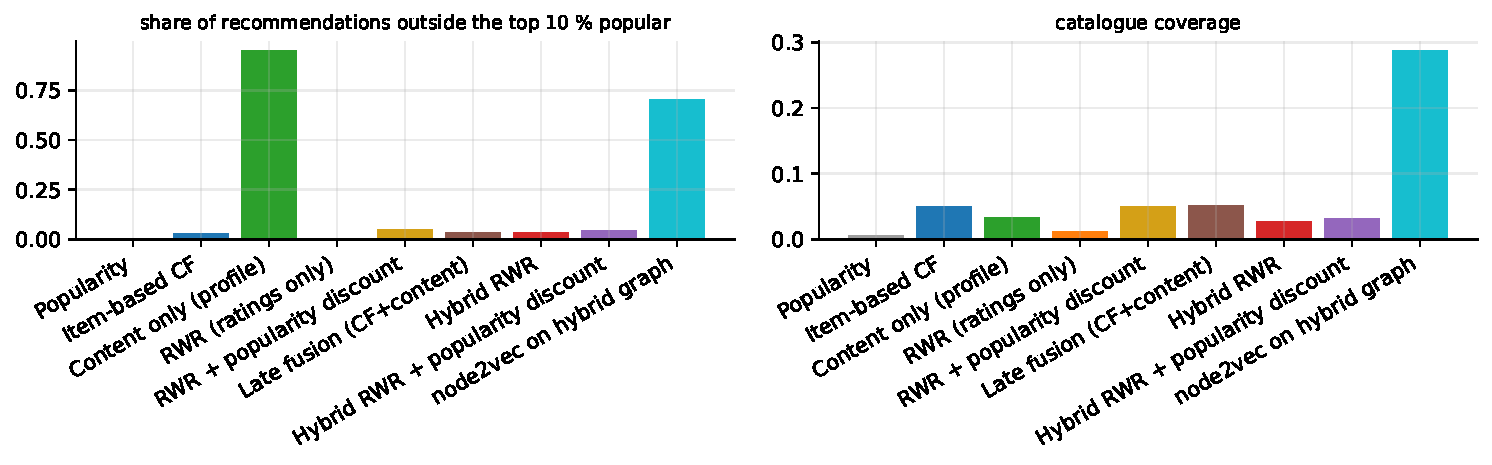
\includegraphics[width=.9\linewidth]{fig_popularity}\hfill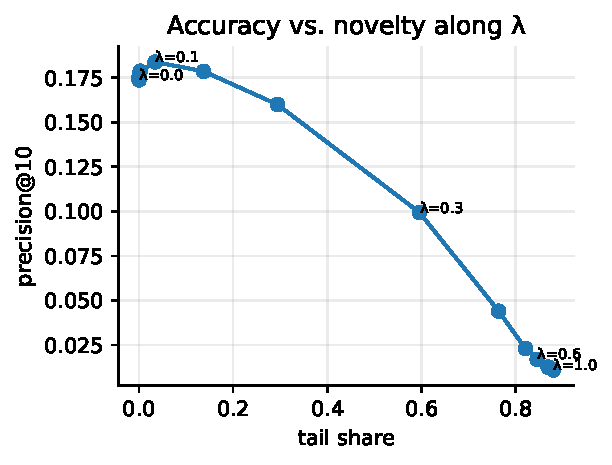
\includegraphics[width=.35\linewidth]{fig_tradeoff}
\caption{Left: tail share and coverage per method. Right: accuracy vs.\ tail share along $\lambda$.}\label{fig:pop}\end{figure}

\textbf{Yes: the accurate methods recommend almost only popular films.} Item-based CF has only $2.9\%$ of its recommendations outside the top-10\,\% most-rated films, the ratings-only RWR $0\%$ (its coverage is just $1.2\%$ of the catalogue) and the hybrid at $\lambda=0.1$ $3.4\%$. The two methods that do reach the long tail (content only: $95\%$; node2vec: $70\%$) are inaccurate on warm films. A popularity discount increases the tail share (to $5.2\%$) and \emph{raises} accuracy, so part of the popularity concentration of plain RWR is an artefact of the walk (stationary mass $\propto$ degree) rather than a signal of taste. Along $\lambda$ (\cref{fig:pop}, right), accuracy and novelty trade off beyond $\lambda\approx0.1$. The data are themselves concentrated ($60\%$ of ratings on $10\%$ of films), which caps what an accuracy-oriented evaluation can reward: recommending popular films is partly correct.

\subsection{Communities of taste (Q4)}
Projecting the user--film graph onto users (cosine of mean-centred rating vectors, each user joined to their $15$ most similar users) gives a user network where Louvain \citep{blondel2008} finds $6$ communities (sizes $158,123,101,95,85,48$; modularity $Q=0.41$; $61\%$ of the similarity weight lies inside communities). The communities are found from ratings only, never from genres. Do they follow genres? We compared the between-community spread of the genre profiles (share of liked films per genre) with $2000$ random relabelings that keep community sizes: observed $1.03$ vs.\ permutation mean $0.15$ (s.d.\ $0.04$), $z=20.7$, $p=5\cdot10^{-4}$ (the smallest value possible with $2000$ permutations). So the communities differ strongly in genre mix (\cref{fig:comm,tab:comm}): e.g.\ C1 over-represents Western ($1.96\times$) and War, C3 Film-Noir ($3.35\times$) and Horror, C0 IMAX/Animation/Fantasy, C2 Documentary/Mystery/Crime. But the communities are not simply ``one genre each'': the normalised mutual information between community and a user's single dominant genre is only $0.066$ (permutation mean $0.029$), because almost every user's top genre is Drama or Comedy; the differences are in the \emph{secondary} genres.

\begin{figure}[H]\centering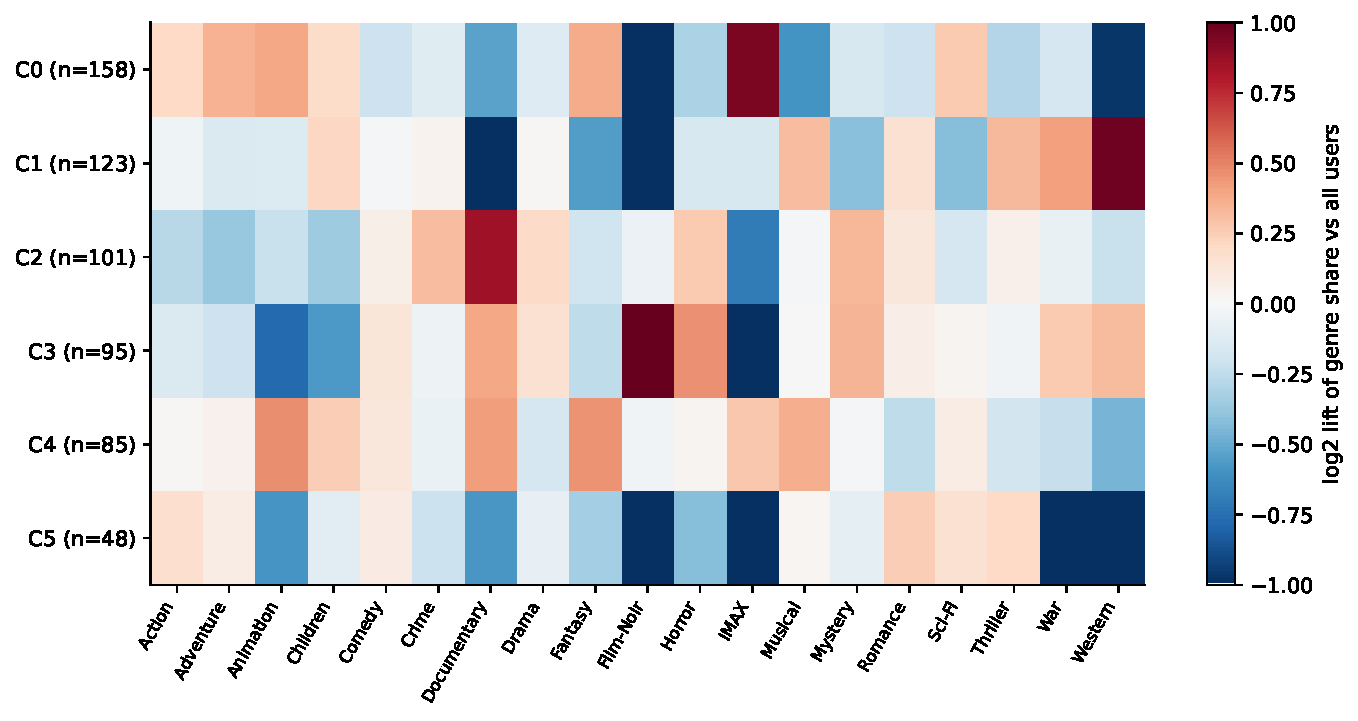
\includegraphics[width=.95\linewidth]{fig_communities}
\caption{Genre over/under-representation (log$_2$ lift) in each user community.}\label{fig:comm}\end{figure}
\begin{table}[H]\centering\footnotesize\begin{tabular}{llp{5cm}p{4cm}}
\toprule
community & users & over-represented genres & under-represented \\
\midrule
C0 & 158 & IMAX (1.92×), Animation (1.31×), Fantasy (1.30×) & Western (0.51×), Film-Noir (0.41×) \\
C1 & 123 & Western (1.96×), War (1.33×), Thriller (1.25×) & Documentary (0.40×), Film-Noir (0.24×) \\
C2 & 101 & Documentary (1.80×), Mystery (1.26×), Crime (1.24×) & Adventure (0.77×), IMAX (0.62×) \\
C3 & 95 & Film-Noir (3.35×), Horror (1.37×), Documentary (1.31×) & Animation (0.58×), IMAX (0.21×) \\
C4 & 85 & Animation (1.38×), Fantasy (1.36×), Documentary (1.34×) & Romance (0.84×), Western (0.73×) \\
C5 & 48 & Romance (1.19×), Thriller (1.15×), Action (1.12×) & Film-Noir (0.36×), IMAX (0.24×) \\
\bottomrule
\end{tabular}
\caption{Communities of at least 20 users and their characteristic genres.}\label{tab:comm}\end{table}

\subsection{Demo}\label{sec:demo}
We use all ratings (no hidden test set) and the hyper-parameters validated on split~0 ($c=0.7$, $\lambda=0.1$).

\paragraph{(a) One user, every method side by side.} User~105 rated \emph{3 Idiots} and \emph{Taare Zameen Par} highly (the example of the brief). \Cref{tab:demo} shows the top 10 of each method (number of ratings in brackets). Item-based CF and the plain walk give mainstream blockbusters (\emph{Star Wars}, \emph{Toy Story}, \emph{Jurassic Park}); the hybrid at $\lambda=0.1$ is close to the walk with some reordering; the popularity-discounted hybrid swaps a few blockbusters for slightly less-rated films (e.g.\ \emph{The Big Lebowski}, with 106 ratings); \emph{content only} returns films on similar subjects that almost nobody rated ($1$--$8$ ratings), and node2vec returns only such obscure films. This is the accuracy--novelty picture of \cref{fig:pop} for one user.

\begin{table}[H]\centering\tiny
\resizebox{\linewidth}{!}{\begin{tabular}{lp{2.6cm}p{2.6cm}p{2.6cm}p{2.6cm}p{2.6cm}p{2.6cm}}
\toprule
 & Item-based CF & RWR (ratings) & Content only & Hybrid RWR & Hybrid + pop. discount & node2vec \\
\midrule
1 & Truman Show, The (1998)  [125] & Star Wars: Episode V - The Empire Strikes Back (1980)  [211] & The Way (2010)  [2] & Star Wars: Episode V - The Empire Strikes Back (1980)  [211] & Star Wars: Episode V - The Empire Strikes Back (1980)  [211] & My Bloody Valentine (1981)  [1] \\
2 & Big Lebowski, The (1998)  [106] & Star Wars: Episode VI - Return of the Jedi (1983)  [196] & In This World (2002)  [2] & Star Wars: Episode VI - Return of the Jedi (1983)  [196] & Star Wars: Episode VI - Return of the Jedi (1983)  [196] & Rivers and Tides (2001)  [1] \\
3 & Star Wars: Episode V - The Empire Strikes Back (1980)  [211] & Toy Story (1995)  [215] & Way, Way Back, The (2013)  [4] & Toy Story (1995)  [215] & Toy Story (1995)  [215] & Bakuman (2015)  [1] \\
4 & Monty Python and the Holy Grail (1975)  [136] & Back to the Future (1985)  [171] & Fun (1994)  [1] & Back to the Future (1985)  [171] & Back to the Future (1985)  [171] & Night Guards (2016)  [1] \\
5 & Signs (2002)  [63] & Monty Python and the Holy Grail (1975)  [136] & Jump In! (2007)  [1] & Jurassic Park (1993)  [238] & Monty Python and the Holy Grail (1975)  [136] & Asterix and the Vikings (Astérix et les Vikings) (2006)  [1] \\
6 & Star Wars: Episode VI - Return of the Jedi (1983)  [196] & Jurassic Park (1993)  [238] & Ex, The (2007)  [1] & Lion King, The (1994)  [172] & Truman Show, The (1998)  [125] & War Dance (2007)  [1] \\
7 & Back to the Future (1985)  [171] & Truman Show, The (1998)  [125] & Beautiful (2000)  [2] & Monty Python and the Holy Grail (1975)  [136] & Lion King, The (1994)  [172] & Hot Girls Wanted (2015)  [1] \\
8 & King Kong (2005)  [40] & Lion King, The (1994)  [172] & Enough Said (2013)  [2] & Truman Show, The (1998)  [125] & Big Lebowski, The (1998)  [106] & Sherlock Holmes: Terror by Night (1946)  [1] \\
9 & Ferris Bueller's Day Off (1986)  [109] & Princess Bride, The (1987)  [142] & Without a Clue (1988)  [1] & Die Hard (1988)  [145] & Jurassic Park (1993)  [238] & Kizumonogatari Part 1: Tekketsu (2016)  [1] \\
10 & Hellboy (2004)  [41] & Die Hard (1988)  [145] & [REC] (2007)  [8] & Indiana Jones and the Last Crusade (1989)  [140] & Princess Bride, The (1987)  [142] & The Blue Planet (2001)  [2] \\
\bottomrule
\end{tabular}
}
\caption{Top-10 recommendations of each method for user 105 (in brackets: number of ratings of the film).}\label{tab:demo}\end{table}

\paragraph{(b) A new film with no ratings.} We add films that are \emph{not in the data set}, described as a catalogue would (title, genres, a few tags), embed the text, link them to their $20$ nearest films and run the hybrid walk from every user. Collaborative methods cannot score these films at all (score exactly $0$ for all users); the hybrid reaches all $610$ users. Scores are compared \emph{within each user's shelf of new releases} (the $680$ films from 2015 on, as in the cold-start evaluation), and users are ranked by the percentile of the new film on their shelf. \Cref{tab:newfilm} checks the choice against \emph{anchor films} a sensible match should have liked: the top-20 users for \emph{Toy Story~4} ($75\%$ liked a Toy Story film vs.\ $28\%$ of all users; its content neighbours are \emph{Toy Story}, \emph{Toy Story 3}, \emph{Toy Story 2}) and for \emph{John Wick: Chapter 3} ($10\%$ vs.\ $3\%$) are clearly enriched in the expected audiences. For \emph{Dangal} the text gives poorer neighbours (\emph{Bollywood/Hollywood}, \emph{The Wrestler} but also \emph{Krabat}, \emph{Special}), because the dataset has only a few Indian films and our text has no synopsis; the enrichment ($20\%$ vs.\ $8\%$ liking an Indian anchor film) is lower but still $2.4\times$ chance.

\begin{table}[H]\centering\small\begin{tabular}{lcccc}
\toprule
new film & top-20 users who liked an anchor film & all users & lift & median percentile of top-20 \\
\midrule
Toy Story 4 (2019) & 75\% & 28\% & 2.7x & 1.2\% \\
John Wick: Chapter 3 (2019) & 10\% & 3\% & 3.0x & 6.5\% \\
Dangal (2016) & 20\% & 8\% & 2.4x & 24.3\% \\
\bottomrule
\end{tabular}

\caption{New films: share of the 20 top-ranked users who liked at least one anchor film, vs.\ all users.}\label{tab:newfilm}\end{table}

\paragraph{(c) Hide a real film and recover its audience.} To get ground truth we hid \emph{all} ratings of five famous films (with a random $10\%$ of films as a pool) and asked which users the hybrid would send each film to (\cref{tab:hidden}). Over the five films the hybrid finds on average $3.0$ real fans among its top 10 users, vs.\ $2.0$ expected by chance and $1.6$ for item-CF (whose ranking is arbitrary on films without ratings). This is a small sample (5 films) and is only an illustration; the quantitative estimate over $365$ cold films is the user-side lift of \cref{tab:cold} ($2.9\times$).

\begin{table}[H]\centering\small\begin{tabular}{lcccc}
\toprule
hidden film & users who liked it & expected by chance (of 10) & hybrid hits (of 10) & item-CF hits (of 10) \\
\midrule
Shrek (2001) & 114 & 1.9 & 2 & 2 \\
Toy Story 2 (1999) & 56 & 0.9 & 2 & 1 \\
Matrix, The (1999) & 222 & 3.6 & 4 & 4 \\
Lion King, The (1994) & 115 & 1.9 & 4 & 0 \\
Gladiator (2000) & 117 & 1.9 & 3 & 1 \\
\bottomrule
\end{tabular}

\caption{Hidden famous films: how many of the 10 users chosen by each method really liked the film.}\label{tab:hidden}\end{table}


%--------------------------------------------------------------------------------------
\section{Discussion}\label{sec:disc}
\paragraph{What does each kind of edge contribute?} Rating edges carry nearly all of the warm accuracy: content only reaches $0.003$ and $\lambda\ge0.5$ is far worse than $\lambda=0$. Content edges contribute (i)~a modest but consistent regularisation gain on warm films at $\lambda\approx0.1$ ($+0.010$ precision@10), and (ii)~\emph{all} the cold-start ability: without them cold films cannot be reached and the recommender is at chance; with them recall is $3.4\times$ chance, already at $\lambda=0.02$. Hence the hybrid is no worse than CF where CF works, and works where CF fails.

\paragraph{Popularity and the interaction between remedies.} The walk's stationary mass is proportional to degree, so the plain RWR is a ``popular-films-in-the-neighbourhood'' recommender. Dividing by $(1+n_i)^{\beta}$ is the cheapest improvement we found (precision $0.174\to0.197$), larger than the content gain. Combining both in our grid-tuned model gave $0.187$ only, because the validation procedure preferred a tiny $\beta$ when content edges were already adding obscure films. A better combination (e.g.\ discounting only the mass arriving through rating edges) is a natural next step.

\paragraph{Limitations.} (1)~\emph{latest-small} is small ($610$ users); standard deviations over splits are about $0.005$, so differences below $\approx0.01$ should be read with care. Our $\lambda$ gain is of that size but is consistently positive in each split. (2)~Content text is short, and many films have no tags; the tag genome of MovieLens-25M would give richer content edges and probably a larger warm-film gain; we did not use it. (3)~The relevance of the hidden data is incomplete (a film not rated is not necessarily disliked), which penalises recommendations of obscure films. (4)~Random-walk scores are not comparable across users, so the user-side cold-start metric uses rank percentiles. (5)~node2vec uses first-order walks with little tuning. (6)~Hyper-parameters were tuned on a coarse grid.

\paragraph{Originality.} Beyond the brief we contribute: three-way verification of the RWR; the degree-discounted walk as an answer to the popularity question; a late-fusion baseline to test whether the graph form matters; cold start in both directions (films-per-user and users-per-film); a permutation test for the genre structure of communities; and a $\lambda$--$k$--$c$ robustness study.

\section{Conclusions}
A single graph with rating edges and content edges, explored by a random walk with restart, gives a recommender that is as accurate as item-based CF on warm films (and slightly better with $\lambda\approx0.1$: precision@10 $0.184$ vs.\ $0.174$), and recommends cold films with $3.4\times$ the recall of chance. Content must be a minor ingredient ($\lambda\le0.15$) for accuracy but a very small amount is enough for cold start. Popular films dominate all accurate recommenders; a degree discount reduces this and improves accuracy. Taste communities exist and differ significantly in genre mix.

%--------------------------------------------------------------------------------------
\section*{Tools, GenAI declaration and contributions}
\textbf{GenAI:} Claude Code (Anthropic, Claude Sonnet 5.5) was used to help write the code in \texttt{src/} and the notebook, and to draft this report. The design, the experiments and the interpretation were checked by the authors. \textbf{Libraries:} numpy, scipy, pandas, scikit-learn, NetworkX \citep{hagberg2008}, matplotlib, PyTorch \citep{paszke2019}, sentence-transformers \citep{reimers2019}. \textbf{Data:} MovieLens latest-small \citep{harper2015}. \textbf{Member contributions:} \emph{[to be filled in by the group]}.

\begin{thebibliography}{99}\small
\bibitem[Linden et~al.(2003)]{linden2003} G.~Linden, B.~Smith, J.~York. Amazon.com recommendations: item-to-item collaborative filtering. \emph{IEEE Internet Computing}, 7(1):76--80, 2003.
\bibitem[Fouss et~al.(2007)]{fouss2007} F.~Fouss, A.~Pirotte, J.-M.~Renders, M.~Saerens. Random-walk computation of similarities between nodes of a graph with application to collaborative recommendation. \emph{IEEE TKDE}, 19(3):355--369, 2007.
\bibitem[Harper and Konstan(2015)]{harper2015} F.~M.~Harper, J.~A.~Konstan. The MovieLens datasets: history and context. \emph{ACM TiiS}, 5(4):19, 2015.
\bibitem[Page et~al.(1999)]{page1999} L.~Page, S.~Brin, R.~Motwani, T.~Winograd. The PageRank citation ranking: bringing order to the web. Stanford InfoLab TR, 1999.
\bibitem[Reimers and Gurevych(2019)]{reimers2019} N.~Reimers, I.~Gurevych. Sentence-BERT: sentence embeddings using Siamese BERT-networks. \emph{EMNLP-IJCNLP}, 2019.
\bibitem[Grover and Leskovec(2016)]{grover2016} A.~Grover, J.~Leskovec. node2vec: scalable feature learning for networks. \emph{KDD}, 2016.
\bibitem[Perozzi et~al.(2014)]{perozzi2014} B.~Perozzi, R.~Al-Rfou, S.~Skiena. DeepWalk: online learning of social representations. \emph{KDD}, 2014.
\bibitem[Blondel et~al.(2008)]{blondel2008} V.~D.~Blondel, J.-L.~Guillaume, R.~Lambiotte, E.~Lefebvre. Fast unfolding of communities in large networks. \emph{J.\ Stat.\ Mech.}, P10008, 2008.
\bibitem[Hagberg et~al.(2008)]{hagberg2008} A.~Hagberg, D.~Schult, P.~Swart. Exploring network structure, dynamics, and function using NetworkX. \emph{SciPy}, 2008.
\bibitem[Paszke et~al.(2019)]{paszke2019} A.~Paszke et~al. PyTorch: an imperative style, high-performance deep learning library. \emph{NeurIPS}, 2019.
\end{thebibliography}
\end{document}
